\begin{figure}
\centering

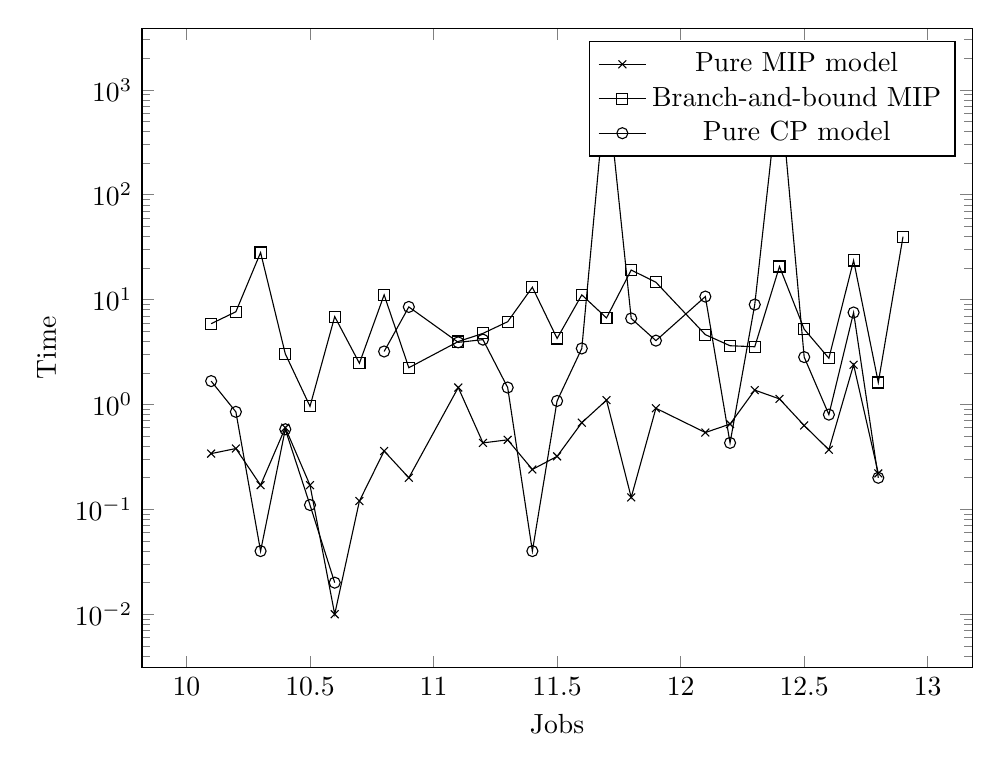
\begin{tikzpicture}
  \begin{semilogyaxis}[xlabel=Jobs, ylabel=Time, width=\textwidth,
  height=0.8\textwidth]
  \addplot[color=black, mark=x ] coordinates { % MIP model times
(10.1, 0.34)
(10.2, 0.38)
(10.3, 0.17)
(10.4, 0.6)
(10.5, 0.17)
(10.6, 0.01)
(10.7, 0.12)
(10.8, 0.36)
(10.9, 0.2)
(11.1, 1.45)
(11.2, 0.43)
(11.3, 0.46)
(11.4, 0.24)
(11.5, 0.32)
(11.6, 0.67)
(11.7, 1.1)
(11.8, 0.13)
(11.9, 0.92)
(12.1, 0.54)
(12.2, 0.65)
(12.3, 1.37)
(12.4, 1.13)
(12.5, 0.63)
(12.6, 0.37)
(12.7, 2.39)
(12.8, 0.22)
  };
  \addlegendentry{Pure MIP model}
  \addplot[color=black, mark=square] coordinates {
(10.1, 5.89)
(10.2, 7.65)
(10.3, 28.09)
(10.4, 3.04)
(10.5, 0.96)
(10.6, 6.88)
(10.7, 2.47)
(10.8, 11.09)
(10.9, 2.24)
(11.1, 3.98)
(11.2, 4.76)
(11.3, 6.15)
(11.4, 13.11)
(11.5, 4.26)
(11.6, 11.09)
(11.7, 6.68)
(11.8, 19.14)
(11.9, 14.62)
(12.1, 4.63)
(12.2, 3.63)
(12.3, 3.55)
(12.4, 20.67)
(12.5, 5.22)
(12.6, 2.76)
(12.7, 23.62)
(12.8, 1.62)
(12.9, 39.76)
  };
  \addlegendentry{Branch-and-bound MIP}
  \addplot[color=black, mark=o] coordinates {
(10.1, 1.67)
(10.2, 0.85)
(10.3, 0.04)
(10.4, 0.58)
(10.5, 0.11)
(10.6, 0.02)

(10.8, 3.2)
(10.9, 8.51)
(11.1, 3.91)
(11.2, 4.15)
(11.3, 1.45)
(11.4, 0.04)
(11.5, 1.08)
(11.6, 3.42)
(11.7, 1200)
(11.8, 6.61)
(11.9, 4.06)
(12.1, 10.68)
(12.2, 0.43)
(12.3, 8.96)
(12.4, 1200)
(12.5, 2.83)
(12.6, 0.8)
(12.7, 7.53)
(12.8, 0.2)
};
  \addlegendentry{Pure CP model}
  \end{semilogyaxis}
\end{tikzpicture}

\caption{Comparison of CPU time used by different models.}
\label{fig:comp_times}
\end{figure}

